\documentclass{acm_proc_article-sp}

\usepackage{graphicx}
\usepackage{epsfig}
\usepackage{subcaption}

\usepackage{amssymb}
\usepackage{amsmath}
\usepackage[utf8]{inputenc}
\usepackage{hyperref}
\usepackage{url}
\usepackage{enumitem}

\begin{document}

\title{Novelty Detection in Text Streams}

\numberofauthors{2} 

\author{
% 1st. author
\alignauthor
Klemen Kenda \\
       \affaddr{Jožef Stefan International Postgraduate School}\\
       \affaddr{Jamova cesta 39}\\
       \affaddr{Ljubljana, Slovenia}\\
       \email{klemen.kenda@ijs.si}
% 2nd. author
\alignauthor
Erik Novak \\
       \affaddr{Jožef Stefan International Postgraduate School}\\
       \affaddr{Jamova cesta 39}\\
       \affaddr{Ljubljana, Slovenia}\\
       \email{erik.novak@ijs.si}
}

\date{15 Feb 2017}

\maketitle
\begin{abstract}
In this report, we describe an approach of using $k$-Nearest Neighbors algorithm for novelty detection. We present the methodology and test the model on several news article data sets acquired by a news analyzing system. We then attempt to evaluate the model using a small sample data set and find that the model is quite effective at detecting novelty in news articles. The model is also publicly available on an online project hosting service and can be executed in an interactive JavaScript playground.
\end{abstract}

\category{I.2.7}{Natural Language Processing}{Text analysis}[novelty detection]

\keywords{$k$-Nearest Neighbors, Novelty Detection, Anomaly Detection, Event Registry} 

\section{Introduction}
With the development of digital media space in the last decades the users nowadays are overloaded with an immense load of information. A massive number of news articles is created every day. A lot of these articles are related to the same events. User only needs to be aware of the first article describing the event and can dismiss the subsequent ones. Finding out which articles contain the same content can make the whole user experience better and much more effective.

Additionally, because of the massive number of data generated every day, storing all of the data became a problem. When regarding text documents, this problem can be solved by storing only novel documents. For this to work, an efficient novelty detecting method is crucial. Novelty detection is the identification of new or unknown data that a machine learning method previously did not come across.

In this report we present an approach of using the $k$-Nearest Neighbors method for detecting novel news articles. We have also created a prototype which was evaluated on a collection of news articles acquired using the Event Registry service\footnote{\url{http://eventregistry.org}}. The prototype uses only plain-text news for extraction of relevant features. Novel articles are detected using the proposed $k$-Nearest Neighbors anomaly detection approach, which can  easily adjust the model with new data from a stream. The prototype implementation is available on GitHub\footnote{\url{https://github.com/klemenkenda/NoveltyDetection}} and can be also be tested on RunKit\footnote{\url{https://runkit.com/klemenkenda/58983987dbfac2001413239a}}. 

The remainder of the report is organized as follows. In section \ref{section:related-work} we present the related work. Section \ref{section:data-description} describes the data used for the analysis, how it was acquired and also how it was preprocessed. In section \ref{section:methodology} we present the developed methodology. Sections \ref{section:results} and \ref{section:evaluation} talk about the the results and their evaluation, respectively. Finally, we conclude our analysis in section \ref{section:conclusion}.

% TODO: runkit bi lahko pokazal kakšno dodatno vizualizacijo
%  - porazdelitev člankov glede na alarme
%  - mogoče odvisnost št. alarmov glede na kriterije (rate)

\section{Related Work}\label{section:related-work}
The topic of novelty detection has been around for some time. A lot of different approaches were described in research papers, where they used Support Vector Machines \cite{clifton2014probabilistic, scholkopf1999support}, $k$-Nearest Neighbors \cite{liao2002use} and other heuristic and statistical approaches.

A heuristic approach was taken in \cite{karkali2013efficient}, where they presented a novelty detection algorithm based on the inverse document frequency scoring function. They relied on the hypothesis that novel documents contain different terms which is then shown in the scoring function.

There are also overview reports on the topic of novelty detection. An example of such report is \cite{pimentel2014review}, where they presented a collection of different novelty detection methods that have been used in research papers in the last decade. The methods were clustered based on the their approach.

\section{Data Acquisition}\label{section:data-description}
The data used for our analysis was acquired using Event Registry \cite{Leban:2014:ERL:2567948.2577024}, a system that can analyze news articles. It collects and processes articles from more than 100k news sources globally in over ten languages, identify and disambiguate named entities mentioned in the articles and identify global events. Event Registry gathers world news with the help of NewsFeed \cite{trampus2012internals}, which is a clean, continuous, real-time aggregated stream of semantically enriched news articles.

\textbf{Crawling.} Event Registry created a Python package which allows the user to query its database for news articles. With it we can query for single articles or for articles that are part of an event or concept. We wrapped this package into a class called \texttt{ERReader}. The methods supported by this class are:

\begin{itemize}[leftmargin=0pt]
\item[] \texttt{\_\_init\_\_(perpage, days)} \\
Setups the class variables, reads the username and password from the \texttt{settings.json} file (corresponding to the Event Registry specifications), connects to Event Registry and logs in. Additionally, it sets how many articles per page will be retrieved and how long is the maximum retrieval interval.

\item[] \texttt{get\_articles\_period(concept, startdate, enddate)} \\
The method retrieves articles containing the given \texttt{concept} for the time period specified by \texttt{startdate} and \texttt{enddate}. It uses the \texttt{get\_articles} method.

\item[] \texttt{get\_articles(concept, startdate, enddate)} \\
This method checks for available articles containing the given \texttt{concept} for the time interval specified by \texttt{startdate} and \texttt{enddate}. It starts article loading by pages using the \texttt{get\_ar\-ti\-cles\_page} method.

\item[] \texttt{get\_articles\_page(concept, startdate, enddate, pagenum)} \\
The method loads the page of articles that contain the \texttt{concept} within the time interval defined by \texttt{startdate} and \texttt{enddate}. 
The page is specified by the \texttt{pagenum} parameter.

\item[] \texttt{print\_articles(list)} \\
It prints a list of the articles date and time to the standard output.

\item[] \texttt{save\_articles(file\_name)} \\
The method saves the retrieved articles to a JSON file, specified by the \texttt{file\_name} parameter. Articles are stored in the Event Registry format (see Figure \ref{fig:dataset}), one article per line.
\end{itemize}

Using this class we were able to simply retrieve news articles for a selected time period, that include a particular concept and were written in a given language. Articles are stored in the Event Registry format.

\textbf{Data Description.}
We retrieved news articles for the four concepts that were published between 2014-01-01 and 2017-02-01. Table \ref{table:concept-stats} shows the number of news articles found for each concept in that time period.

% TODO: do we use Slovene (?), how is it with stopwords
\begin{table}[!htb]
	\centering
    \begin{tabular}{|l|c|c|r|}
    	\hline
    	Concept Name & Language & Instances & File Size \\
        \hline
        Borut Pahor         & Slovene & 8410   & 49MB \\
        Borut Pahor         & English & 3160   & 17MB \\
        Peter Prevc         & Slovene & 3127   & 16MB \\
        Peter Prevc         & English & 742    & 3.5MB \\
        Microsoft           & English & 155576 & 1.3GB \\
        European Commission & English & 221736 & 1.9GB \\
        \hline
    \end{tabular}
    \caption{The retrieved news articles statistics. Two of the concepts were crawled for both Slovene and English articles. The most news articles were found for the European Commission concept, followed by the Microsoft concept.} \label{table:concept-stats}
\end{table}

 An example of an article is shown in Figure \ref{fig:dataset}.

\begin{figure}[!htb]
\centering
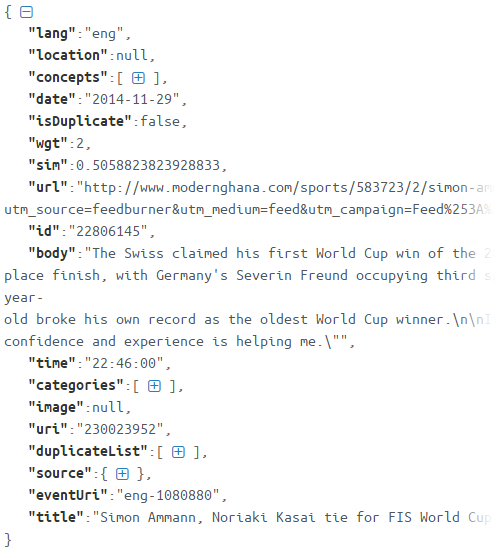
\epsfig{file=dataset.png, width=8.5cm}
\caption{Example record from EventRegistry. The record contains article information such as its title, content and language in which the article was written, the time and date of its publication, the categories in which the article falls and other.}
\label{fig:dataset}
\end{figure}

% CHECK: data understanding not needed?

% \textbf{Preprocessing.}
% % TODO: check, write better
% The news data were preprocessed using the QMiner data processing platform \cite{qminer}. We have used \texttt{featureSpace} functionality to calculate different n-gram weights (TFIDF, TF, IDF and none), we have used built-in stop-words for English (and ??? Slovene), we have used the Porter stemmer. We have checked different number of n-grams (1 to 5) and normalization. 

\section{Methodology}\label{section:methodology}
Here we present an approach for detecting novel news articles. This approach might also be used for other types of text documents, such as scientific articles or tweets.

\textbf{Method.}
We considered the use of $k$-Nearest Neighbors ($k$NN) method. It is a non-parametric method, that can be used for different machine learning tasks such as classification and regression \cite{altman1992knn}. Because this method does no computation in the training phase, it is a so called lazy learner method. 

We used a slightly adjusted $k$NN method for novelty detection. With it we would calculate similarity of the new article to those that the model has already seen. If the similarity is smaller than the threshold we specified at the start of the evaluation, we label the article as novel and  store it in the model. We can specify multiple thresholds that represent different novelty levels. With this we can express the severity of the novelty.


\textbf{Features.}
Each article is represented by a bag-of-words model using 2-grams.
Then we remove stop words depending on the language the articles are written in. Here, stop words are short function words like the, which, on etc.
After that, we use Porter stemming to reduce inflected words to their word stem base or root form.

Finally, we use TF-IDF to calculate the weights of the terms in the articles. TF stands for Term Frequency and counts the number of times the term occurs in the article while IDF stands for Inverse Document Frequency, which is a measure of how much information the term provides to the document, e.g. if the term is common or rare across all articles. The TF-IDF weights are calculated as the product of Term Frequency and Inverse Document Frequency. 

We used only the articles body to generate the feature sets. 

\textbf{Implementation.}
The novelty detection model was created using the QMiner data processing platform \cite{qminer}. The platform contains a stream aggregator called 
\texttt{StreamAggrAnomalyDetectorNN} which represents the anomaly detector using the previously described Nearest Neighbors algorithm (with $k$ set to $1$). It calculates the distances of a new example from its nearest neighbors and, depending on the input threshold values, it classifies it as a novelty with an appropriate severity measure. The thresholds used in the model are $0.2$, $0.05$, $0.01$.

\section{Results}\label{section:results}
Direct results from the prototype are very simple. Each article was sent through the model, which assigned the articles novelty level. Articles with a novelty level greater than zero are found novel. The novelty level also depict the magnitude of the articles novelty. An example of the results is depicted in \ref{fig:resultList}.

\begin{figure}[h]
\centering
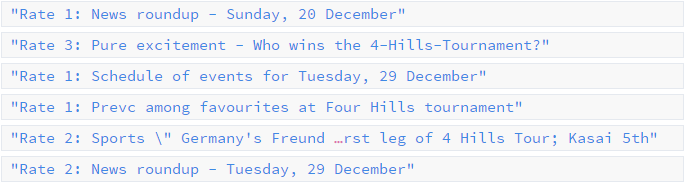
\epsfig{file=resultList.png, width=8.5cm}
\caption{A subset of detected novelties for the Peter Prevc english data set.}
\label{fig:resultList}
\end{figure}

An overview of novelty detection on a the set of selected concepts is shown in Figure \ref{fig:histogram-concepts}. The histograms present the novelty level on the $x$ axis and number of articles on the $y$. We can notice that most of the published articles do not contribute any new information. The number of original articles is much smaller. We can observe that the concepts that appear in media less have a bigger percentage of novelty per article. These are the concepts that are globally less interesting and therefore smaller number of articles are published, which results in relatively higher novelty.

Comparison of two different weight score, TF-IDF and TF, is depicted in \ref{fig:histogram-weights}. We can see that with similar parameters TF is more strict on novelty classification. Quick qualitative analysis showed that TF-IDF gives results, that can be more easily interpreted.
% Razprava?

It is also interesting to compare how a particular concept behaves in local and global news. As concepts we used the names of two well known Slovenians, Borut Pahor and Peter Prevc. Then, for each concept we crawled the articles in both Slovene and English. Results are depicted in Figure \ref{fig:histogram-language}. Firstly, we observed that there are more news about the concepts published in the local media. Secondly, we saw that the fraction of novel articles are comparable between the languages. The exception is the number of the articles with highest novelty level, which seems to be roughly connected to the number of articles regarding a particular concept in a particular language.

In Figure \ref{fig:timelines} we present dynamics of concept occurrences and novelty in the news through time. For sub-figures \ref{fig:rfig1} and \ref{fig:rfig2} our algorithm remembered last 4000 articles, in case of \ref{fig:rfig3} and \ref{fig:rfig4} we only remembered last 200. Novelty in the news related to European Commission (\ref{fig:rfig2}) is quite monotonous. Microsoft generated slightly more dynamic results, however, it is difficult to explain for example a spike in June 2014, as it consists of many different (seemingly) non-related events that can not be generalized. For less frequent concepts like "Peter Prevc" and "Borut Pahor" depicted in figures \ref{fig:rfig3} and \ref{fig:rfig4} we observe that more news usually means more old news (less novelty).

\section{Evaluation}\label{section:evaluation}
The $k$NN method is a descriptive data mining technique which works on unlabeled data. To prepare a proper evaluation a labeled data set would be needed, which was not available. A simple supervised testing method can be performed with a data set with low frequency of articles. News are usually focused on a particular event and different events usually do not overlap. The common dynamics in the stream of news is that we first get the initial news about the event, which the system detects as novel, which is immediately followed by other news about the same event. Many on-line media often take advantage of agency news. This means that the same news article is usually republished with minor content additions and changes.

Example of such a sequence is depicted in Table \ref{tab:tande}. The system detected a new event when it received the first news article (\textit{Ski Jump: Norway's Tande wins season opener}). The model was then able to find sufficient similarities of incoming articles and did not classify them as novel. A week later, the model received a similar article (\textit{Prevc second in Norwegian-dominated ski jumping event}). The article was talking about another event with similar results. Nevertheless, the model correctly classified the article as novel.

A similar example can be observed in Table \ref{tab:germany}. The first news article with the title \textit{Ski jumping: Slovenians open new season with second place} was taken from a Slovenian news site and it focuses on the Slovenian team. The system identified the article as novel. Furthermore, the first international article on the same topic with the title \textit{Sports - Germany wins season's first ski ...} was also identified as novel, but with a lower novelty level, which is correct, as the article presents another the event from another vantage point. Subsequent articles have all been classified as non-novel with the exception of the article focusing on a particular person only (\textit{Ski jumping: Prevc opens season with second place}). 

Same dynamics can be observed throughout the data set. We have manually analyzed 12 such events and discovered that for only 2 events there was at least one article in a sequence that got the wrong novelty level. 

Exceptional articles, those that don't arrive in sequences, are the articles that focus on Peter Prevc as a sportsman, person and his influence on society, articles that focus on a different sport, such as Alpine Skiing, and only briefly mention Peter Prevc and aggregated daily or weekly news. These articles are almost always identified as a novelty, which is correct. Three of such exceptional articles are for example \textit{Prevc setting off mass euphoria, paper says}, \textit{Golden Fox: Rebensburg wins Maribor giant slalom, Slovenia's Drev second} and \textit{Victorious Prevc psychotherapist to Slovenians}. 

In our rough (and we have to stress biased) evaluation, 10 out of 12 events were classified correctly. Within those ten events, there were only 5 out of 103 articles that have been misclassified. A very rough estimation for accuracy is therefore $95\%$, which is  surprisingly good.

%An extensive overview of evaluation of outlier detection with $k$-NN based methods is provided in \cite{Campos2016}, there has been, however, no evaluation done with the method applied to textual data.

\section{Conclusion}\label{section:conclusion}
In this report we presented the $k$-Nearest Neighbors novelty detection approach. We developed and evaluated the prototype on several news data sets acquired using Event Registry. We made several comparisons regarding the weighting score and language. An attempt of a proper evaluation show that the novelty detection model is effective at detecting novel articles. 

Future work includes proper evaluation of the model, which would enable us to tune the model (feature selection, parameter tuning), testing the model on other types of text documents, such as tweets and scientific articles. It would be interesting to check the effect of using LSI or LDA representation of the articles.

% bibliography
\bibliographystyle{abbrv}

\bibliography{textmining}  % textmining.bib is the name of the Bibliography in this case
\balancecolumns

\onecolumn

\appendix
\section{Evaluation of Novelty Detection Model}\label{appendix:streams} % This is Appendix A

\begin{table}[!htb]
	\centering
    \begin{tabular}{|r|l|}
    	\hline
    	Level & Title \\
        \hline
        3 & Ski Jump: Norway's Tande wins season opener \\
        0 & Sports - Tande of Norway wins ski jumping World Cup event; Kasai 5th \\
        0 & Daniel-Andre Tande of Norway wins season's 1st individual ski jumping World Cup \\
        0 & Daniel-Andre Tande of Norway wins ski jumping World Cup \\
        0 & Norwegian ski jumper Tande kicks off season with World Cup win \\
        0 & Daniel-Andre Tande of Norway wins ski jumping World Cup \\
        0 & Daniel-Andre Tande of Norway wins seasons 1st individual ski jumping World Cup \\
        0 & Daniel-Andre Tande of Norway wins ski jumping World Cup \\
        2 & Prevc second in Norwegian-dominated ski jumping event\\
		0 & Prevc second in Norwegian-dominated ski jumping event (adds) \\
        \hline
    \end{tabular}
    \caption{Sequence of articles and their novelty level for the first individual World Cup competition in Ski Jumping (2015/16).}
	\label{tab:tande}
\end{table}
%
\begin{table}[!htb]
	\centering
    \begin{tabular}{|r|l|}
    	\hline
    	Level & Title \\
        \hline
        2 & Ski jumping: Slovenians open new season with second place \\
		0 & Ski jumping: Slovenians open new season with second place (adds) \\
        1 & Sports - Germany wins season's first ski jumping World Cup; Japan 4th \\
        0 & Germany beats Slovenia on home snow to win season's first ski jumping World Cup \\
        0 & Germany wins season's first ski jumping World Cup \\
        0 & Germany wins season's first ski jumping World Cup \\
        0 & Germany wins season's first ski jumping World Cup \\
        0 & Germany wins season's first ski jumping World Cup \\
        0 & Germany beats Slovenia on home snow to win seasons first ski jumping World Cup \\
        1 & Ski jumping: Prevc opens season with second place \\
        0 & News roundup - Sunday, 22 November \\
        \hline
    \end{tabular}
    \caption{Sequence of articles and their novelty level about the first team World Cup competition in Ski Jumping (2015/16).}
	\label{tab:germany}
\end{table}

\section{Novelty Detection on selected Concepts}\label{appendix:selected-concepts} % This is Appendix A


\begin{figure}[!htb]
  \begin{subfigure}{.5\textwidth}
    \centering
    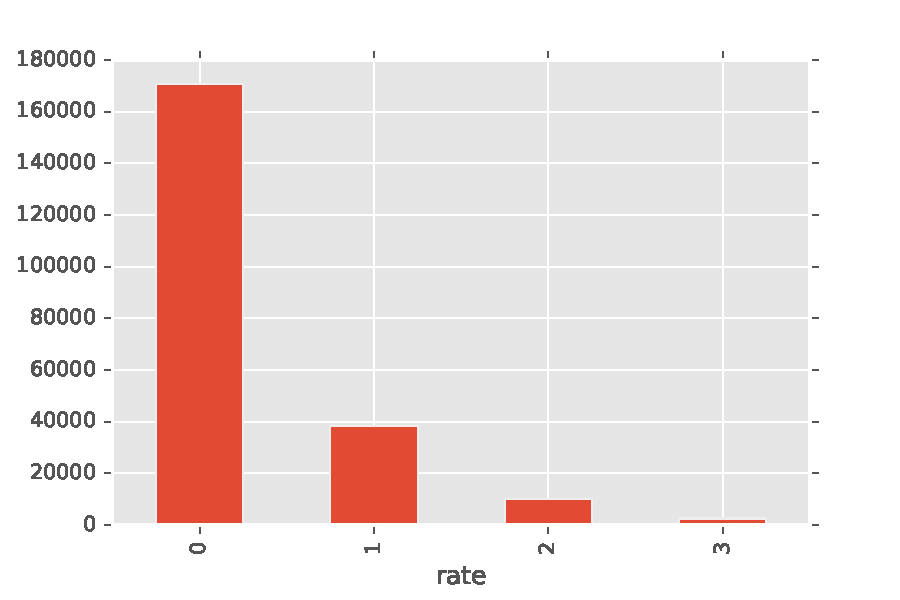
\epsfig{file=histograms/ecENGhist_tfidf.pdf,width=7cm}
    \caption{European Commission (ENG)}
    \label{fig:hfig1}
  \end{subfigure}%
  \begin{subfigure}{.5\textwidth}
    \centering
    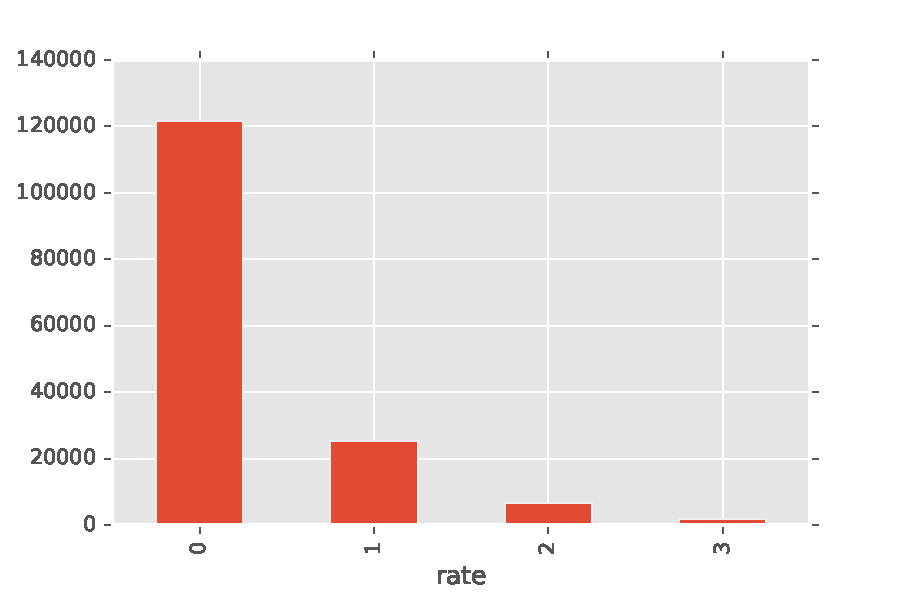
\epsfig{file=histograms/msENGhist_tfidf.pdf,width=7cm}
    \caption{Microsoft (ENG)}
    \label{fig:hfig2}
  \end{subfigure}%
  \\
  \begin{subfigure}{.5\textwidth}
    \centering
    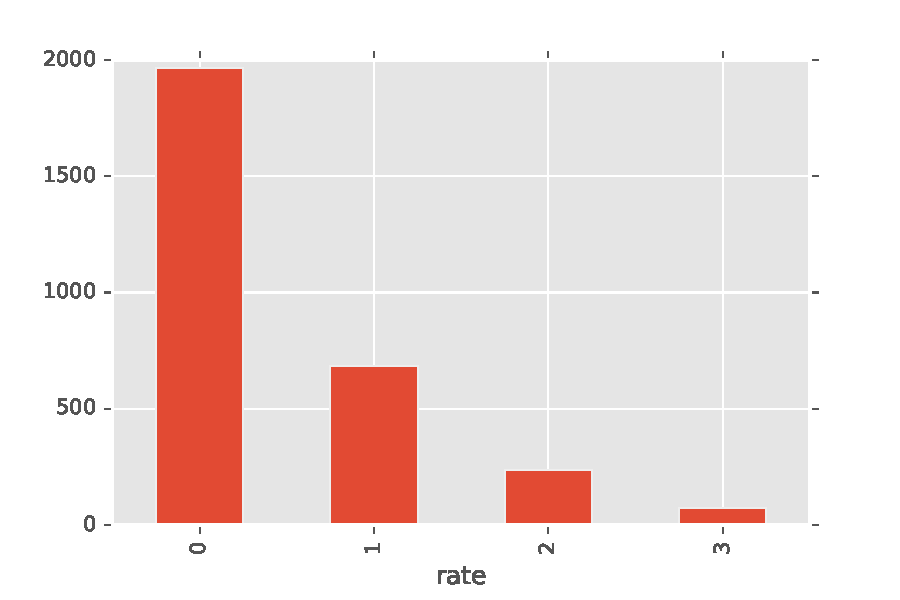
\epsfig{file=histograms/pahorENGhist_tfidf.pdf,width=7cm}
    \caption{Borut Pahor (ENG)}
    \label{fig:hfig3}
  \end{subfigure}%
  \begin{subfigure}{.5\textwidth}
    \centering
    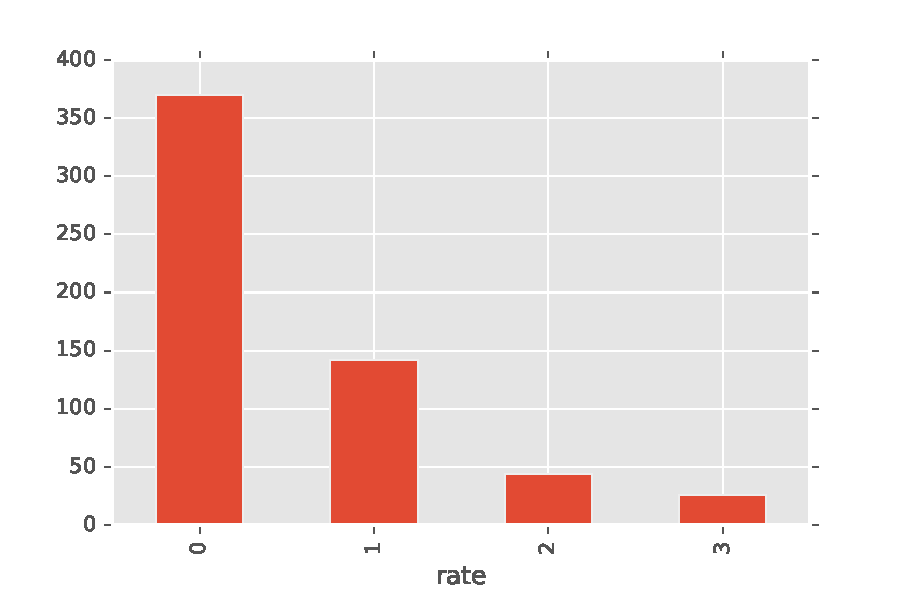
\epsfig{file=histograms/prevcENGhist_tfidf.pdf,width=7cm}
    \caption{Peter Prevc (ENG)}
    \label{fig:hfig4}
  \end{subfigure}%

\caption{The distribution of novelty levels for articles of a particular concept. The analysis uses the TF-IDF term weighting.}
\label{fig:histogram-concepts}
\end{figure}

\begin{figure}[!htb]
  \begin{subfigure}{.5\textwidth}
    \centering
    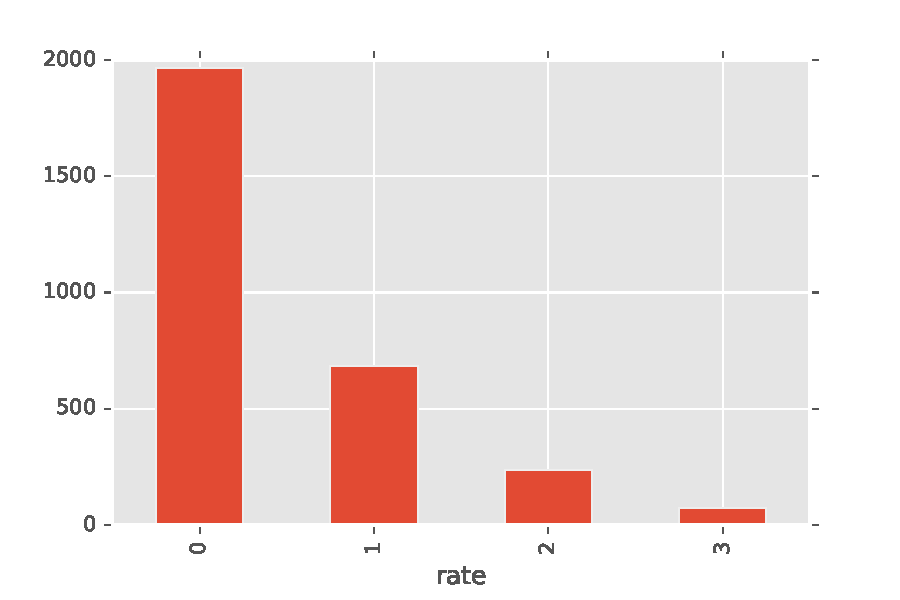
\epsfig{file=histograms/pahorENGhist_tfidf.pdf,width=7cm}
    \caption{Borut Pahor (ENG) - TF-IDF}
    \label{fig:wfig1}
  \end{subfigure}%
  \begin{subfigure}{.5\textwidth}
    \centering
    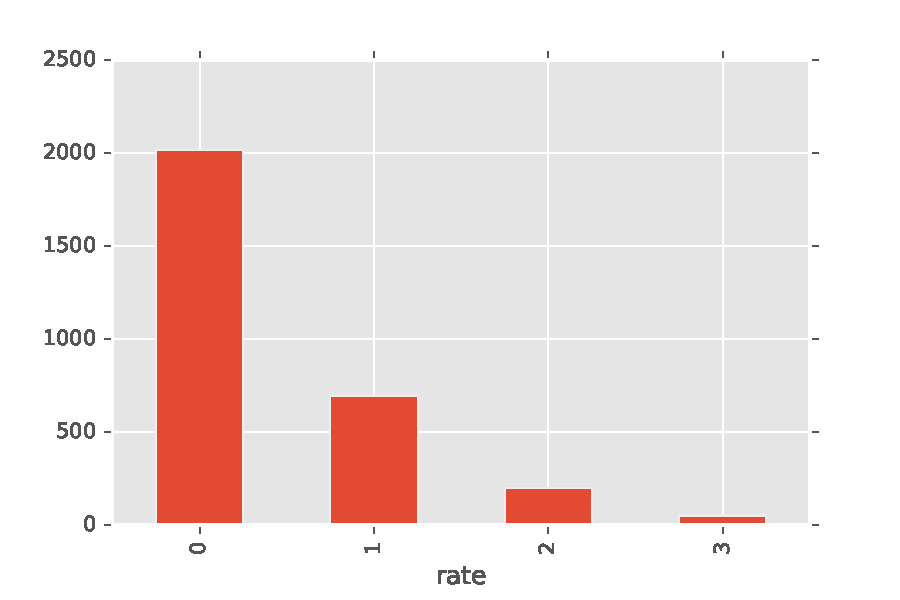
\epsfig{file=histograms/pahorENGhist_tf.pdf,width=7cm}
    \caption{Borut Pahor (ENG) - TF}
    \label{fig:wfig2}
  \end{subfigure}%
  \\
   \begin{subfigure}{.5\textwidth}
    \centering
    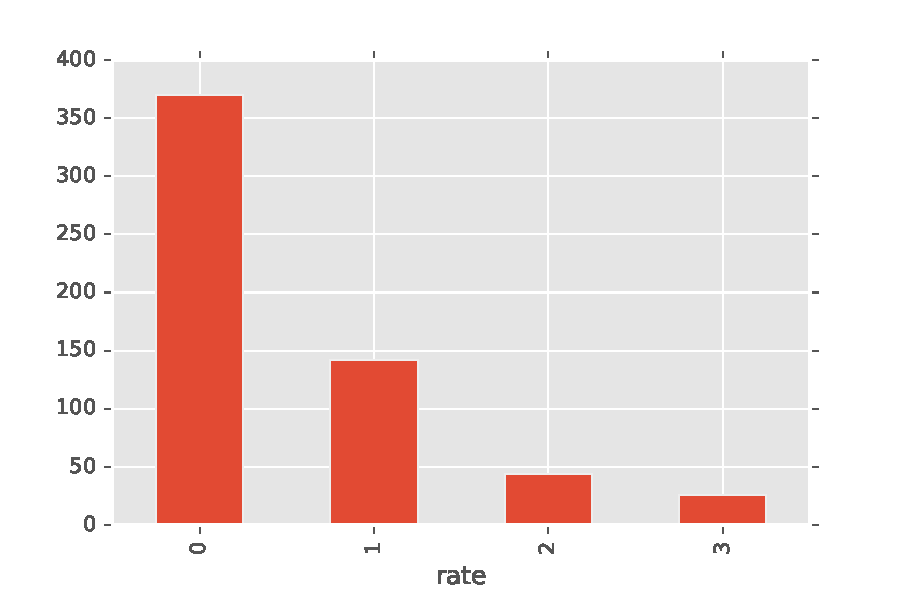
\epsfig{file=histograms/prevcENGhist_tfidf.pdf,width=7cm}
    \caption{Peter Prevc (ENG) - TF-IDF}
    \label{fig:wfig3}
  \end{subfigure}%
  \begin{subfigure}{.5\textwidth}
    \centering
    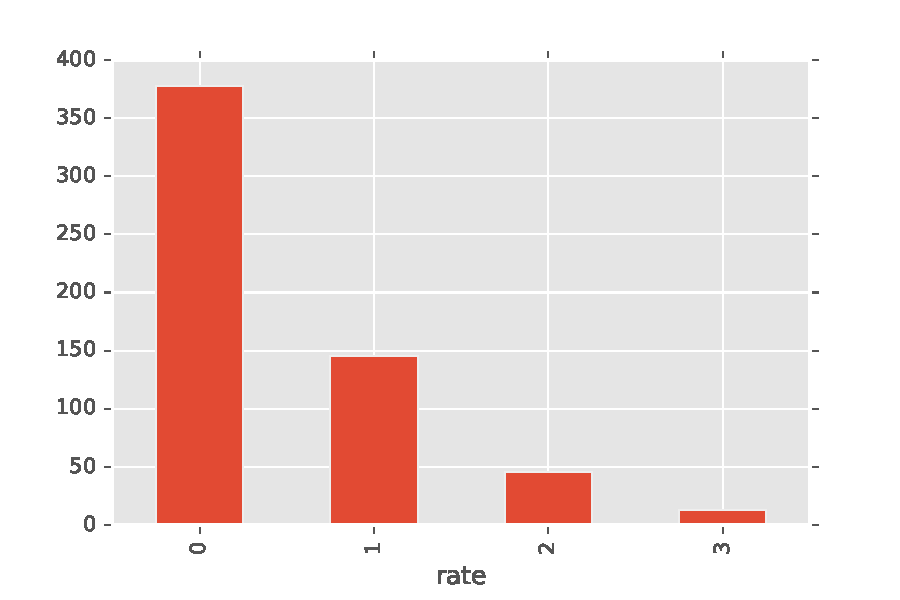
\epsfig{file=histograms/prevcENGhist_tf.pdf,width=7cm}
    \caption{Peter Prevc (ENG) - TF}
    \label{fig:wfig4}
  \end{subfigure}%
\caption{A comparison of novelty level distributions using different term weights.}
\label{fig:histogram-weights}
\end{figure}

\begin{figure}[!htb]
  \begin{subfigure}{.5\textwidth}
    \centering
    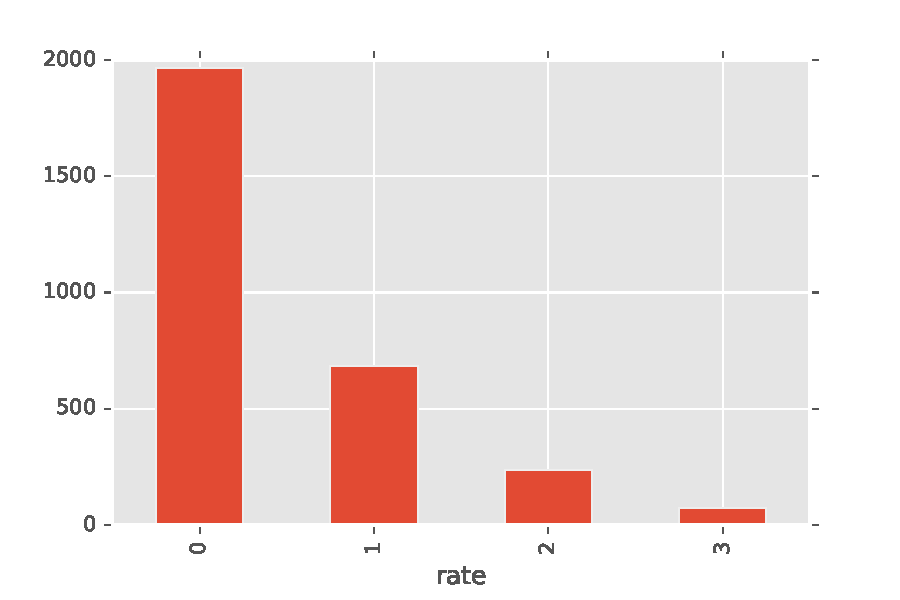
\epsfig{file=histograms/pahorENGhist_tfidf.pdf,width=7cm}
    \caption{Borut Pahor (ENG)}
    \label{fig:lfig1}
  \end{subfigure}%
  \begin{subfigure}{.5\textwidth}
    \centering
    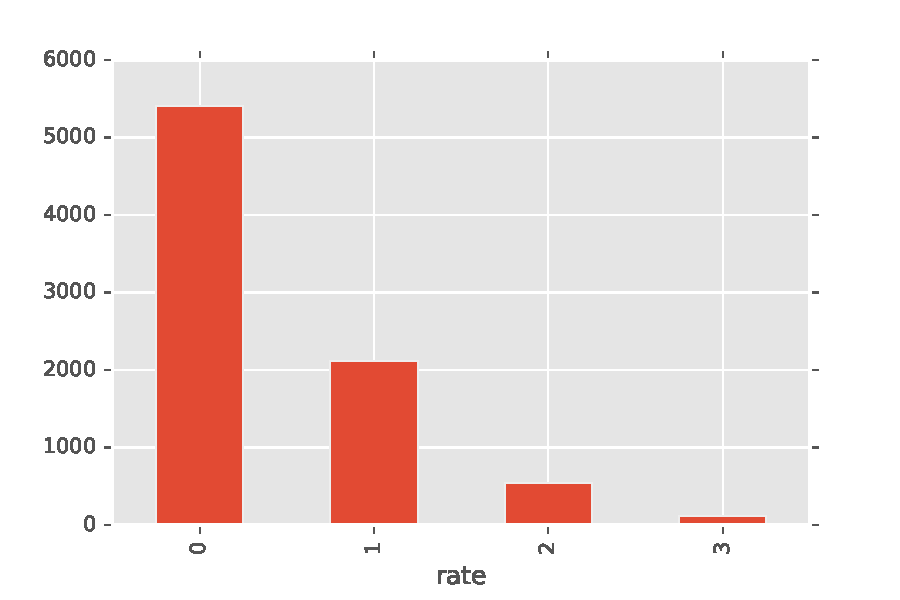
\epsfig{file=histograms/pahorSLVhist_tfidf.pdf,width=7cm}
    \caption{Borut Pahor (SLV)}
    \label{fig:lfig2}
  \end{subfigure}%
  \\
   \begin{subfigure}{.5\textwidth}
    \centering
    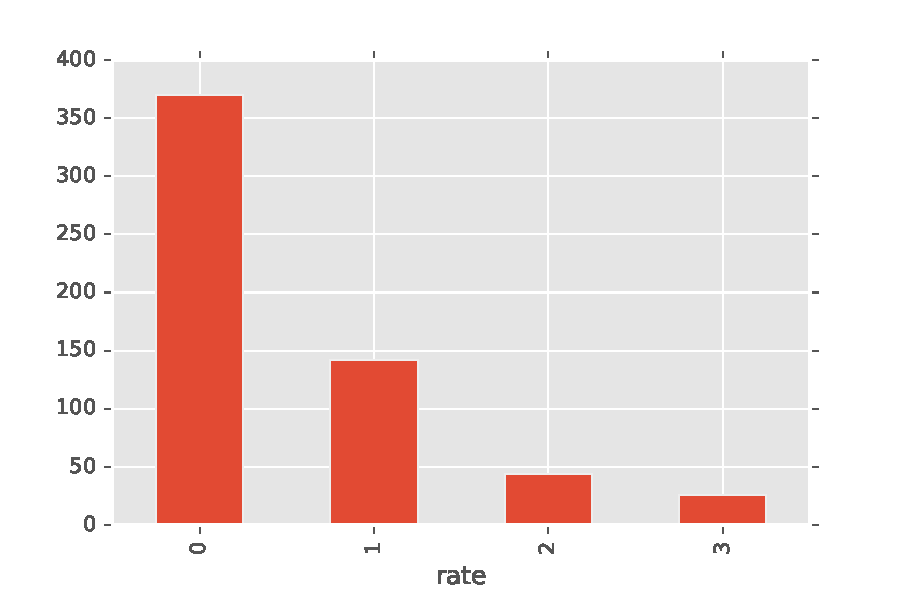
\epsfig{file=histograms/prevcENGhist_tfidf.pdf,width=7cm}
    \caption{Peter Prevc (ENG)}
    \label{fig:lfig3}
  \end{subfigure}%
  \begin{subfigure}{.5\textwidth}
    \centering
    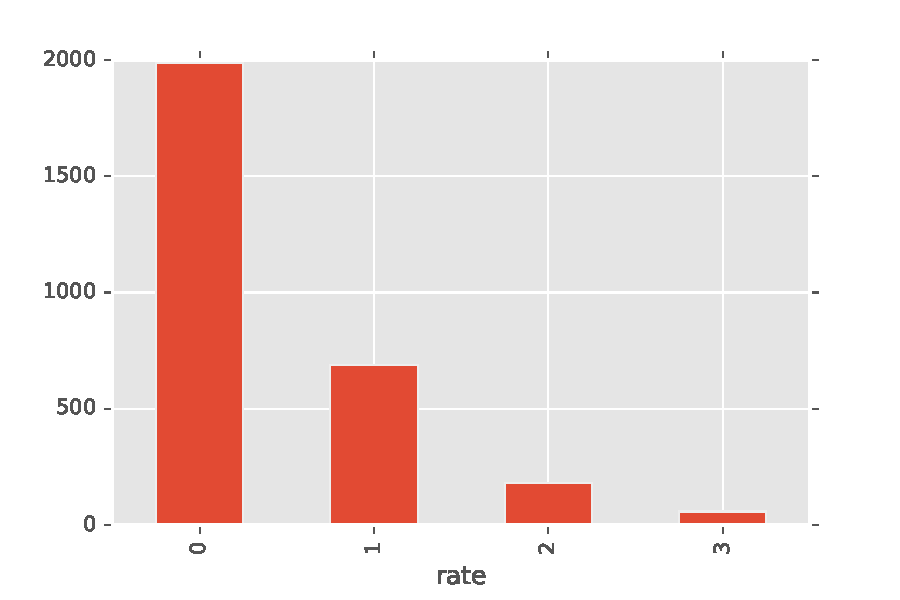
\epsfig{file=histograms/prevcSLVhist_tfidf.pdf,width=7cm}
    \caption{Peter Prevc (SLV)}
    \label{fig:lfig4}
  \end{subfigure}%
\caption{Comparison of novelty rate distributions for Slovenian and English articles. The term weight used is TF-IDF.}
\label{fig:histogram-language}
\end{figure}

\begin{figure}[!htb]
  \begin{subfigure}{.5\textwidth}
    \centering
    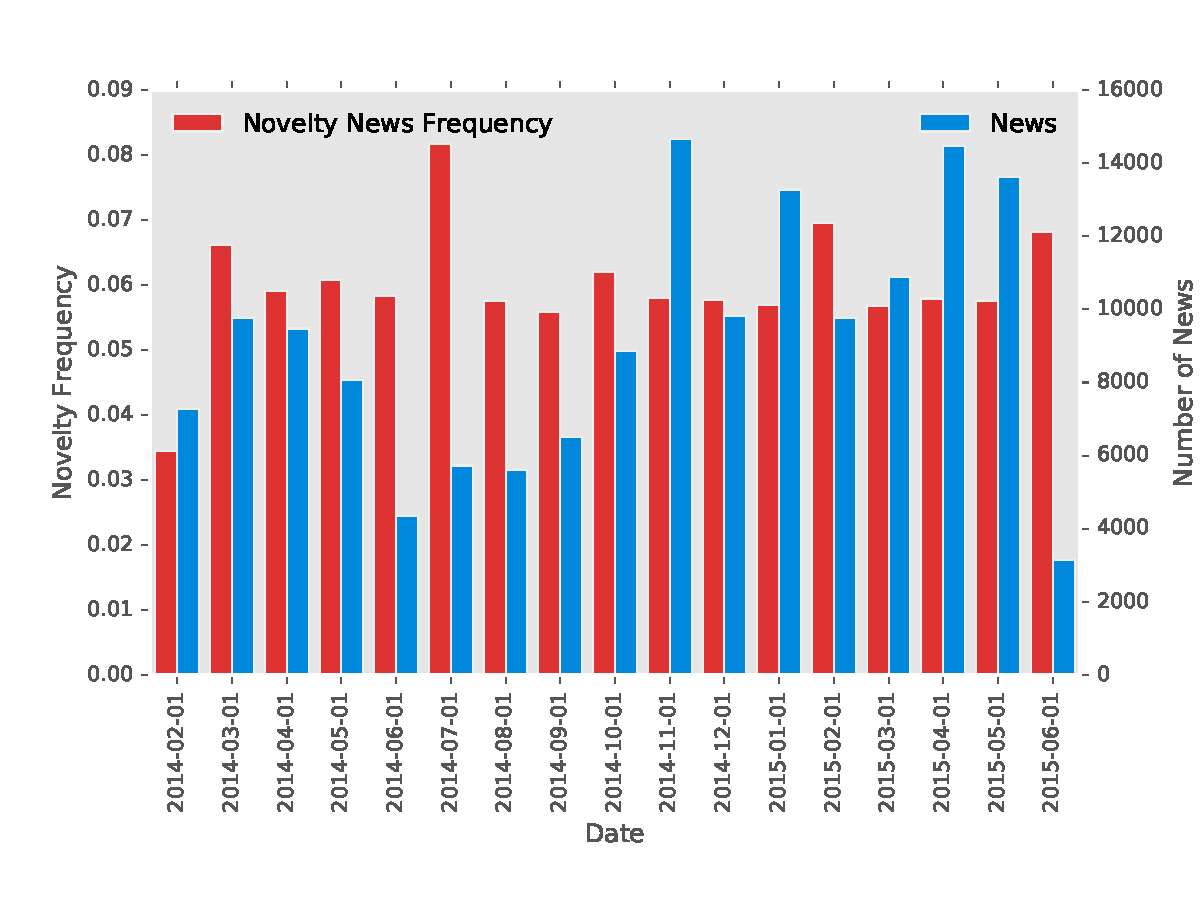
\epsfig{file=rates/msENG_rate.pdf,width=7cm}
    \caption{Microsoft (ENG)}
    \label{fig:rfig1}
  \end{subfigure}%
  \begin{subfigure}{.5\textwidth}
    \centering
    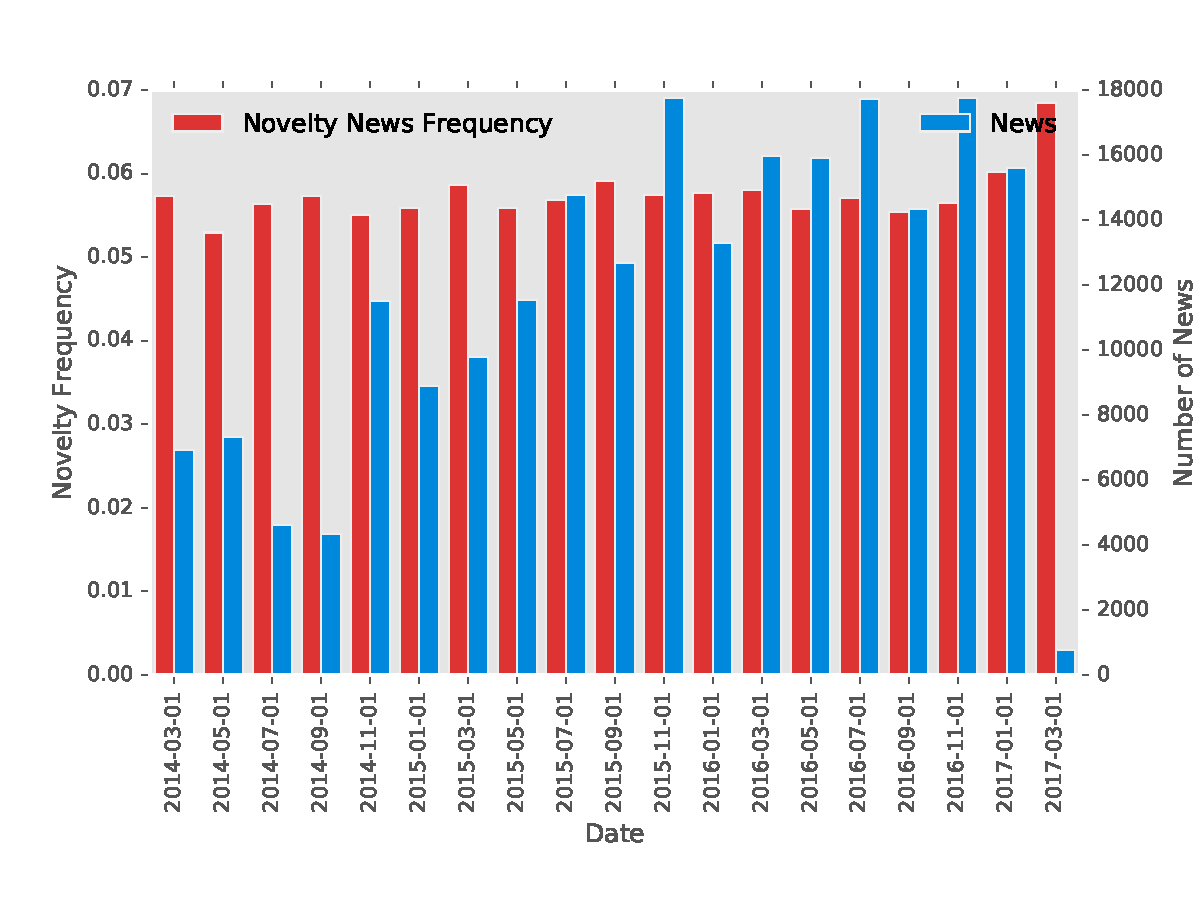
\epsfig{file=rates/ecENG_rate.pdf,width=7cm}
    \caption{European Comission (ENG)}
    \label{fig:rfig2}
  \end{subfigure}%
  \\
   \begin{subfigure}{.5\textwidth}
    \centering
    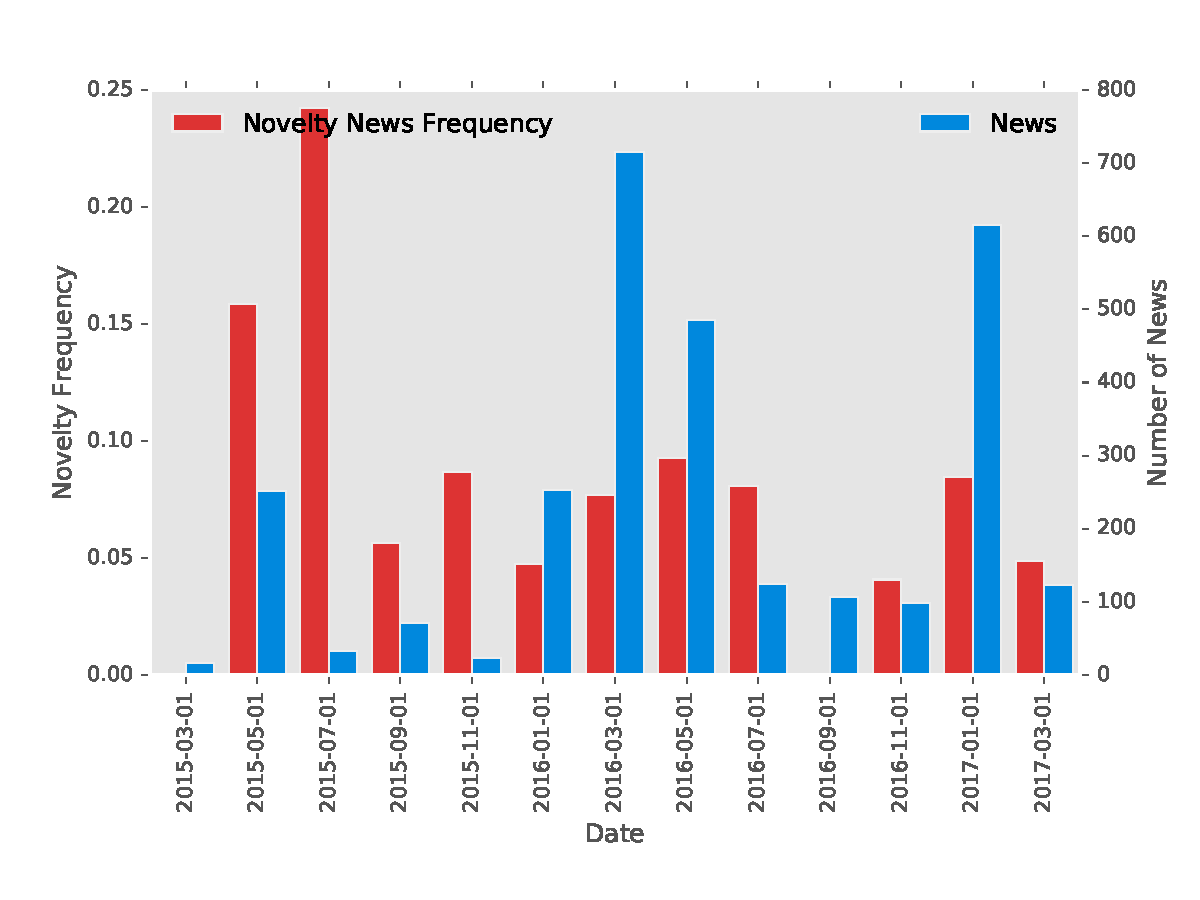
\epsfig{file=rates/prevcSLV_rate.pdf,width=7cm}
    \caption{Peter Prevc (SLV)}
    \label{fig:rfig3}
  \end{subfigure}%
  \begin{subfigure}{.5\textwidth}
    \centering
    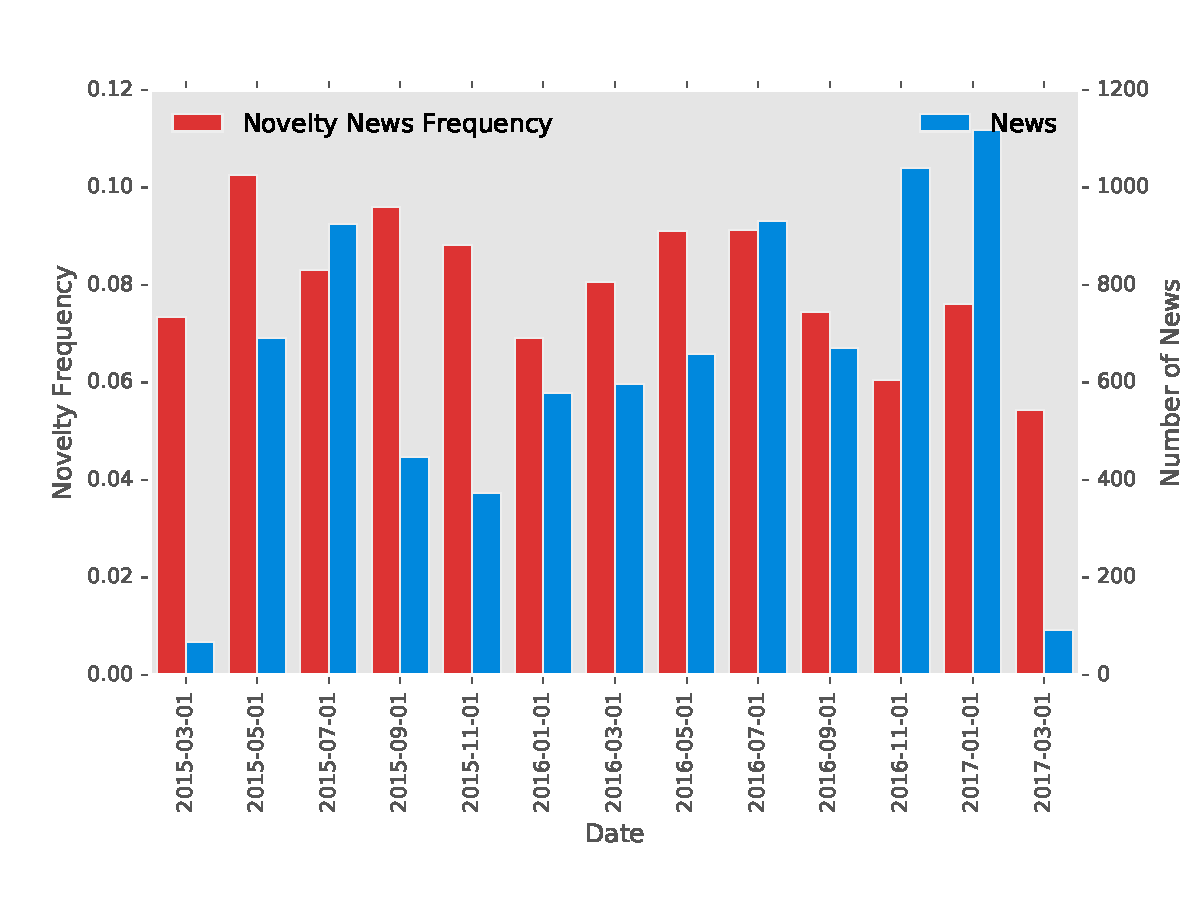
\epsfig{file=rates/pahorSLV_rate.pdf,width=7cm}
    \caption{Borut Pahor (SLV)}
    \label{fig:rfig4}
  \end{subfigure}%
\caption{Novelty detection level through time compared to total number of relevant news articles.}
\label{fig:timelines}
\end{figure}

\text{  }

\end{document}